\chapter{State of the Art} \label{chap:state_of_the_art} % 10-15 pages

This chapter consists of relevant and similar work structured in three parts: First, we present other research of unsupervised generative models for video, that are either novel or are based on V-GAN like our architecture. Then in Section \ref{sec:rel_frame_prediction} future frame prediction approaches are showcased and information on how they could be integrated into IFTM is provided. These architectures are also generative in nature, so the differences and similarities to our solution are discussed as well. Lastly in Section \ref{sec:rel_vad}, an overview on the research of video anomaly detection (VAD) is provided. As these video anomaly detection approaches were evaluated using similar data sets, we also give insight into their respective evaluation methods and how they differ to ours. 



% Video Generation Methods
\section{Video Generation} \label{sec:rel_vgan}

\paragraph{Video Object Segmentation} 
As noted in our presentation of the adapted C-VGAN architecture for next-frame prediction in Section \ref{subsec:vgan_mod_2}, the untangling of the latent spaces of background and foreground stream is not novel. Spampinato et al. in their first proposed approach \cite{spampinato2018vos} built directly on VGAN, copying the architecture (see Section \ref{subsec:vgan_mod}), but utilizing two latent spaces, one for each pathway of the generator: The background's latent space remains the same for the whole generated video, so a 1-dimensional vector is sufficient. For the foreground stream, one vector for each output frame is required. However, as the frames in a video depend on each other, the temporal coherences must be encoded as a trajectory between the different latent points. This can be done using an recurrent neutral network (RNN) encoder. Spampinato et al. utilize LSTM \cite{hochreiter1997long} for this task and the encoder that is attached before the foreground stream is trained alongside the rest of the GAN. This untangling has the advantage that variations in the background latent space result in different general scenes, while allowing the foreground stream to reuse the same motion patterns, if the trajectory latent vectors are the same.

For the discriminator network, it is split into two pathways after the first convolutional neural network (CNN) encoder layers: The first one is the discriminator stream, that does the binary discrimination of real and synthetic videos. The other one performs pixel-wise dense prediction, generating an object segmentation mask and, as a second output, an estimation of the optical flow between the frames in a given video. This two-stream extension, similar to other work for optical flow \cite{simonyan2014two, lai2017semi}, when properly trained in tandem with its counterpart, forces the discriminator to focus on motion patterns and not static discriminating features, thus indirectly improving the quality of the synthetic motion patterns of the foreground generator stream. It also allows the discriminator to be used on its own for object and motion segmentation for video after training has been completed. Hence giving this approach its name (VOS-GAN)\nomenclature{VOS-GAN}{Generative adversarial network for video object segmentation}. To optimize both new tasks, the discriminator loss function is also extended with a function for the evaluation of the optical flow and a comparison between the segmentation mask of the discriminator and the mask that the foreground generator stream produces. In later work \cite{spampinato2019adversarial}, Spampinato et al. extend both adversarial components with so-called 3D residual blocks --- deep residual layers of the same dimensions using 3D convolutions, that feature shortcut connections to pass the output of one layer not to its direct successor, but to one or more layers after that one \cite{he2016deep}. These components allow the construction of deeper networks, because non-residual networks often increase in train and test error when adding more layers. The resulting generator and discriminator network is shown in Figure \ref{fig:vos_gan}. 

\begin{figure}
  \centering	
	\begin{subfigure}{\textwidth}
    \centering
    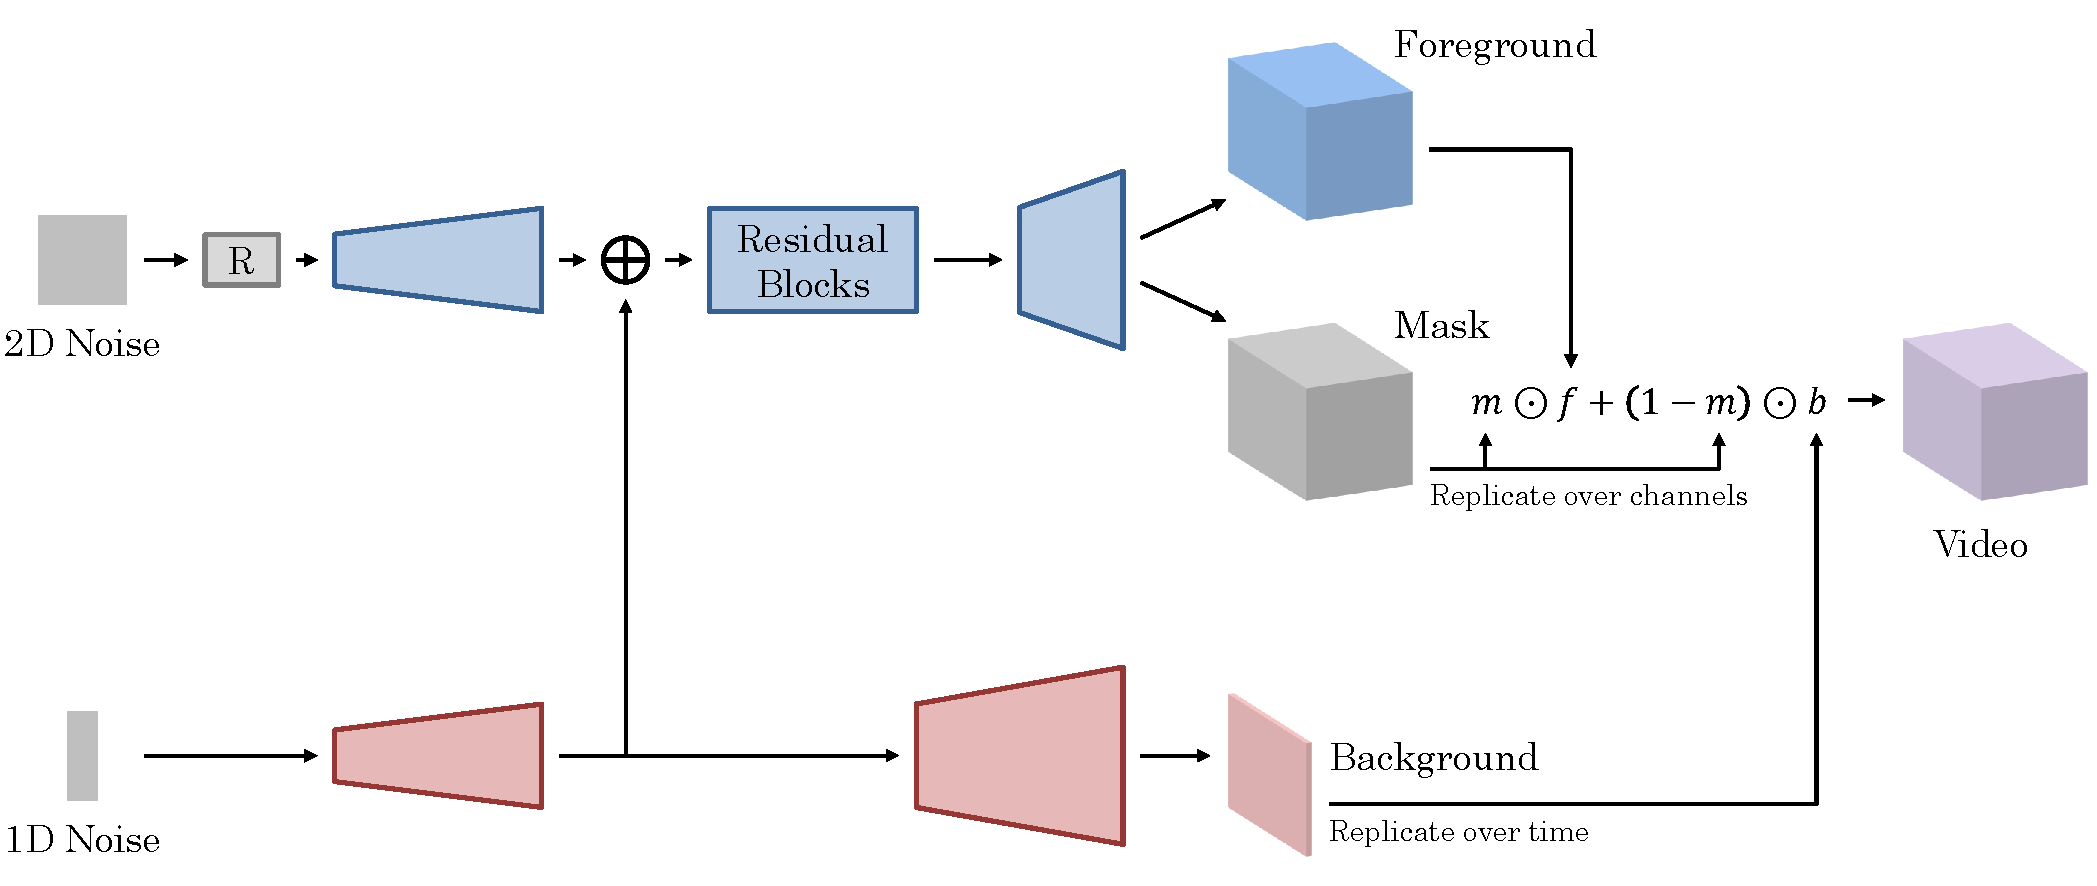
\includegraphics[width=1\textwidth]{graphics/gan/vosgan/vosgan_g.pdf}
    \caption{VOS-GAN generator.}
    \label{subfig:vosgan_g}
  \end{subfigure}
 
	\begin{subfigure}{\textwidth}
    \centering
    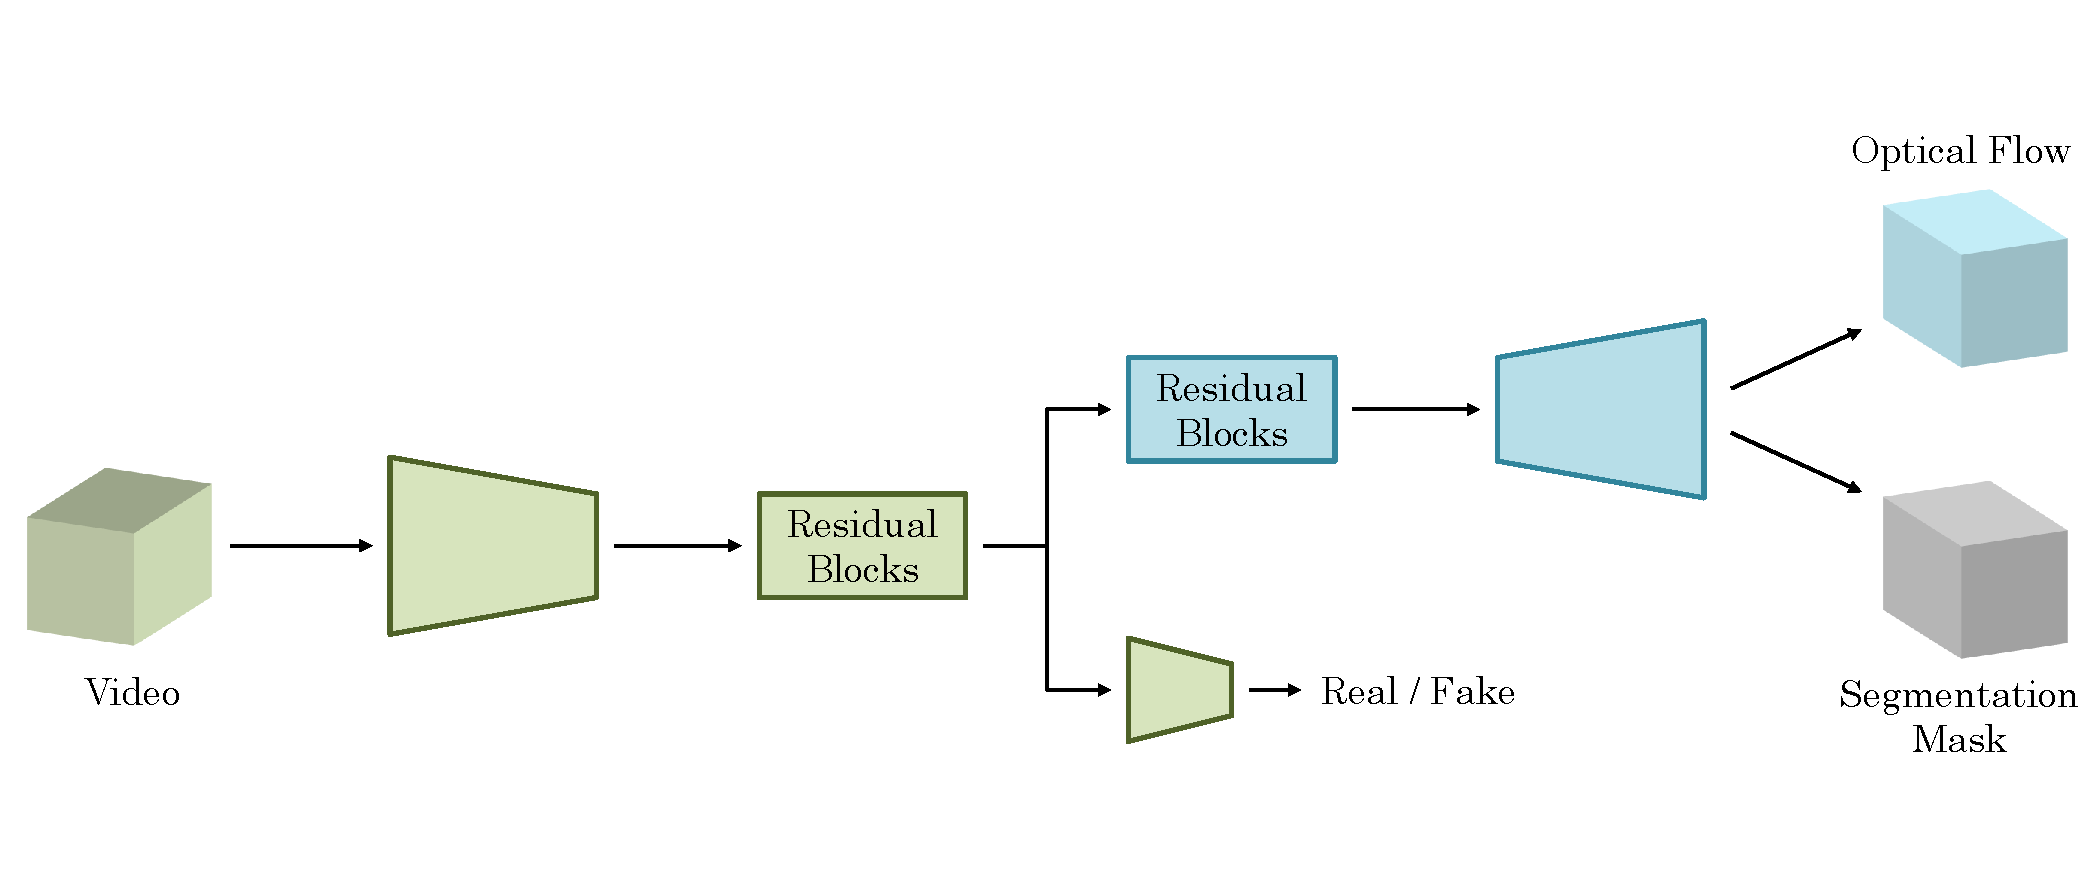
\includegraphics[width=1\textwidth]{graphics/gan/vosgan/vosgan_d.pdf}
    \caption{VOS-GAN discriminator.}
    \label{subfig:vosgan_d}
  \end{subfigure}

  \caption[VOS-GAN architecture.]{VOS-GAN architecture \cite{spampinato2019adversarial}. For the generator in (a), a sequence of latent vectors is randomly sampled and then processed by an RNN ($R$), before being passed to the 3D de-convolutional foreground stream. The foreground and its mask are conditioned on the generated background by concatenation ($\bigoplus$) of intermediate outputs of the spatial de-convolutional background stream. The discriminator in (b), being similar to the one from VGAN, is extended with an extension for the object segmentation (foreground) mask and an optical flow prediction output.}
  \label{fig:vos_gan}
\end{figure}

For evaluation, VOS-GAN was run on parts of the data set provided by Vondrick et al. for the evaluation of VGAN \cite{vondrick2016generating}. Besides evaluating VOS-GAN's performance for object segmentation and action recognition, Spampinato et al. also directly compared its performance to VGAN, utilizing a user preference score system with human workers, and achieving an $80\%$ to $20\%$ preference of VOS-GAN generated videos over VGAN. But while outperforming VGAN and other newer approaches for that task, there is no research on how to adapt VOS-GAN for future frame prediction unlike with VGAN. Most likely, the main challenge lies in the encoder that would project the input frames into their latent representation, so future frames can be extrapolated. Since the trajectory information might be already encoded using preceding 3D convolutions at that point, the RNN encoder is redundant. Although in its original application it was proven to be the crucial improvement to the quality of motion dynamics in the generated videos. Furthermore it is unclear how this extension for the VOS-GAN generator would influence the stability of the training procedure, as our version of the VGAN discriminator had to be severely impaired to guarantee an equilibrium of the losses after adjustments were made.

\paragraph{Motion and Content Decomposition}
Opposed to video generation techniques that generate a whole set of frames of a video from latent space through 3D de-convolutions, there are also ones that generate video output in a step-wise manner: Tulyakov et al. propose a motion and content decomposed generative adversarial network (MoCoGAN)\nomenclature{MoCoGAN}{Motion and content decomposed generative adversarial network} \cite{tulyakov2018mocogan}. Improving on earlier versions of temporal GANs for video \cite{saito2017temporal}, MoCoGAN divides the latent space into two parts, similar to VOS-GAN. However the so-called content subspace, modeled using a Gaussian distribution, contains all objects and the static scene, while the 1-dimensional latent space from VOS-GAN and the background latent space of our approach only include the static object patterns. The second subspace is called the motion latent subspace and describes the motion of the objects in the former subspace. Generated sequentially using an RNN, one can sample from this space and combine the result with a fixed sampling of the content subspace to have a latent vector pair, one for each synthetic video frame. This has the advantage that one can traverse the motion subspace for varying amounts of time, thus creating latent space trajectories of different lengths, which correspond to different long synthetic videos. The actual synthetic output is produced using a frame generator, generating one frame for each vector pair. So when the generated frames of an entire sequence are put together, one has the entire generated video. 

\pagebreak

In addition, similar to the original version of C-VGAN (see Section \ref{subsec:cvgan_mod}), this architecture was modified with an encoder that converts single frames into their content and motion subspace latent representation. So by using that vector in the motion subspace as a starting point for the motion vector sequence that is created through the RNN, one can make future frame predictions. There is also a second discriminator in the architecture, that only does image discrimination. Pairing this model with a separate video discriminator allows the former to focus on static information, while the latter can rate the quality of the motion patterns in a given video. The value function that is optimized during training is adjusted accordingly, weighting image and video discriminator losses equally. Thus, training can be done using an alternating updating procedure, always fixing either the RNN and the video frame generator, or the two discriminators.

\pagebreak

MoCoGAN --- like VOS-GAN, was compared to VGAN but using different data sets. A comparison to C-VGAN for future frame prediction was also performed. The video data had a focus on human actions and close-up human facial expressions. Why VGAN and MoCoGAN were not compared using the former's original data set was not explained. Using these data sets, MoCoGAN had an $84.2\%$ to $15.8\%$ user preference score for generated facial expressions, $75.4\%$ to $24.6\%$ for human poses and actions, and $66.9\%$ to $33.1\%$ for human poses and actions when making future frame predictions from a single image. As with VGAN, future frame prediction was an afterthought, since it is more about image to video translation than actual forecasting. This would require additional modifications to the encoder and the RNN that generates the motion vector sequence to allow the usage of a variable number of past video frames for forecasting.

\paragraph{Flow- and Texture-Based} 
Combining multiple generators to let them specialize in certain tasks, similar to MoCoGAN with the RNN generating the input for the actual image frame generator, is not novel. Ohnishi et al. also utilize this, joining two different GANs, one to model the optical flow and one to generate the corresponding texture, i.e. the synthetic video \cite{ohnishi2017hierarchical}. This flow and texture generative adversarial network (FTGAN)\nomenclature{FTGAN}{Flow and texture generative adversarial network} builds on the idea, like MoCoGAN, that generating encoded information representing the motion pattern is much easier than to create the video directly. For their model to generate the optical flow, they recycle VGAN, but with only its foreground generator stream (see Section \ref{subsec:vgan_mod}). A zero-matrix is given instead of the background stream, since the optical flow should be zero if there are no motion patterns being generated. The second model is a conditional generator (C-GAN, see Section \ref{subsec:cgan}), that encodes a given optical flow into the latent code for another foreground stream. This pathway, also being similar to the one proposed for VGAN, applies multiple 3D de-convolutions to create a foreground and its corresponding spatio-temporal mask. In addition and similar to residual blocks mentioned earlier in this section, Ohnishi et al. utilize skip connections that bridge intermediate outputs from the flow encoder to layers in the texture generator foreground stream, utilizing U-Net architecture \cite{ronneberger2015u}. Second, like in VOS-GAN, encoded information about the content of the background is passed to an intermediate foreground layer, so the foreground is conditioned on that information as well. This is required, since the background is generated from 100-dimensional random latent code, using fractionally-strided spatial convolutions like VGAN, therefore not dependent on the optical flow conditional input. Combination of the three components --- foreground, mask, and the background, is done as in VGAN. 

The respective discriminators for the optical flow and the texture generator are similar to VGAN. With the latter model being extended with an additional 3D convolutional pathway, because the conditional optical flow input needs to be passed to that discriminator as well. Unlike MoCoGAN however, these two GANs are not trained as one, but this is done independently at the beginning. Note that while the flow generator generates synthetic optical flow from 100-dimensional random latent code and does not receive any ground truth information during training, the conditional texture generator gets the ground truth optical flow of to be generated videos. Then in the second training step, the models' updates are joined together --- this is also called joint-training, where the optical flow generator depends on both its own discriminator and also on the discriminator of the texture generator. This refines the models and allows the optical flow generator to create complementary inputs for its successive partner. 

For evaluation, Ohnishi et al. trained both VGAN and FTGAN on human action data sets and then let human workers decide which models' outputs they prefer in terms of realness. The results were mixed though, with roughly even preferences across data sets. However, when utilizing not their optical flow generator but instead a state of the art flow extraction technique \cite{revaud2015epicflow} and passing its outputs to their texture generator, their results improved noticeably, achieving a user preference score of $72\%$ for that generator to $28\%$ for VGAN. This flow-given texture generator in general created video frames of better quality than both VGAN and FTGAN. In addition, when adapting the discriminators of FTGAN for the purpose of action classification, they outperformed the one from VGAN for that task. This was to be expected, since there are two separate discriminators available to learn motion and appearance information, respectively. Finally, there was no attempt made to extrapolate future optical flow for a given video, thus allowing future frame prediction. Such a modification would not require any change of the texture generator though, but only to its preceding optical flow generator.

% Video Frame Prediction Methods
\section{Future Frame Prediction} \label{sec:rel_frame_prediction}

\paragraph{Motion Content Network}
Predating MoCoGAN from the previous section, the motion content network (MCnet)\nomenclature{MCnet}{Motion content network} by Villegas et al. \cite{villegas2017decomposing} is a GAN-based architecture, that, like our proposed modification to C-VGAN to enable next-frame prediction (see Section \ref{subsec:vgan_mod_2}), utilizes two separate encoder streams, but with a few key differences: As depicted in Figure \ref{fig:mc_net}, the motion encoder is an RNN that is able to process spatial information in given frames by using a 2D convolutional version of LSTM \cite{shi2015convolutional}. With the result being a latent representation of the temporal dynamics at the current time step. In addition, compared to our foreground encoder, which receives a fixed number of past frames, MCnet only gets passed the computed difference between the current and the previous frame in the video stream at every time step and recurrently encodes it. The model therefore dynamically determines by itself when to remember or to forget past observations. On the other hand however, for the content encoder --- called the background encoder stream in our architecture, only the frame of the current time step is passed to the model to create the latent representation of the scene. While it reduces the needed complexity for that encoder, it comes at a disadvantage when motion patterns cover static object patterns at some points in the video stream but not in others: Our model is able to cope with that, generating the entire background, and at a later step removing covered static object patterns from it, when they are not needed at certain steps in the predicted video. In VGAN architectures, this can be done using the spatio-temporal mask of the foreground stream. For MCnet this is not a possibility, since that information is unavailable to the content encoder and thus the model has to rely on the motion encoder to capture and encode that information.

\begin{figure}
	\centering
	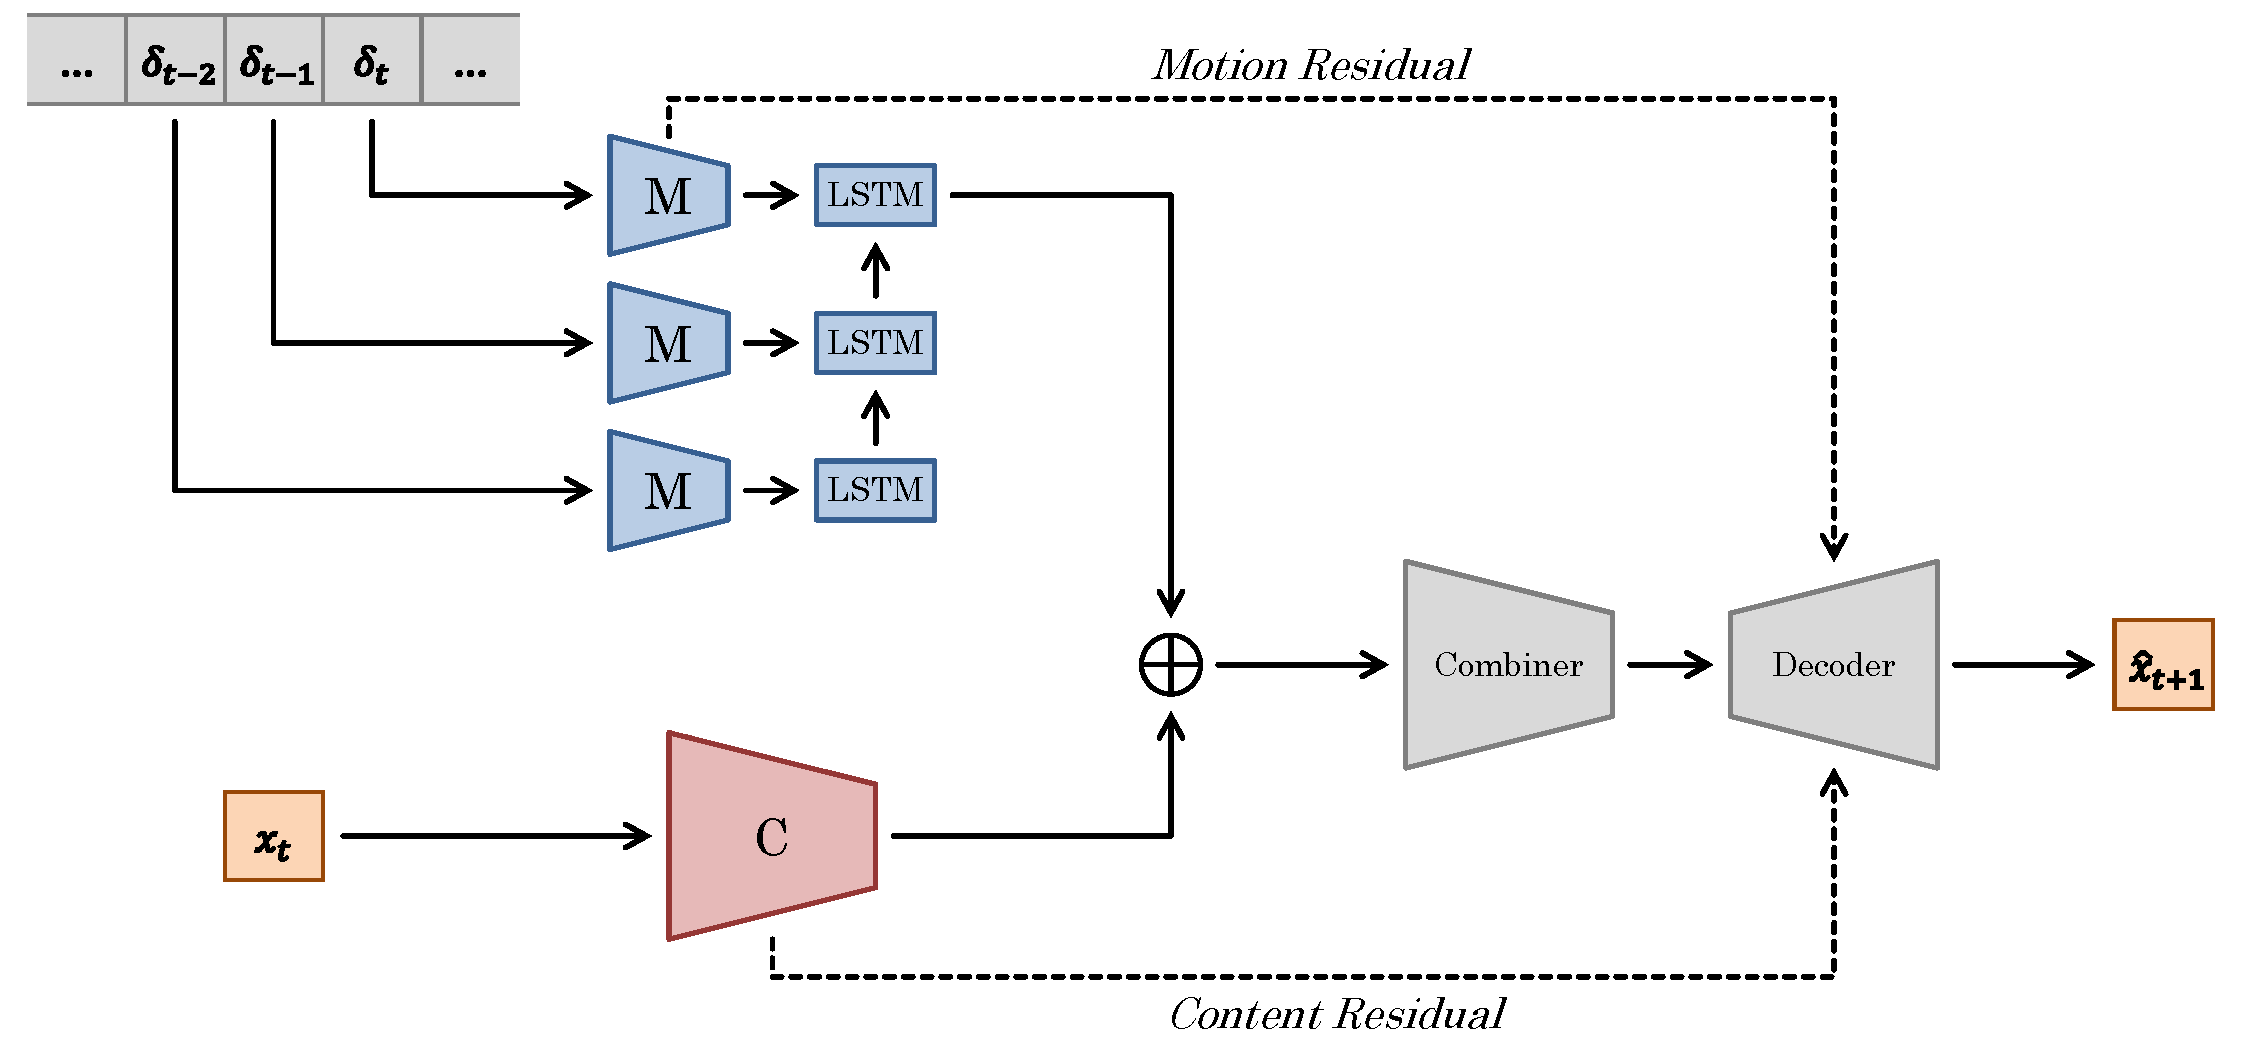
\includegraphics[width=1\textwidth]{graphics/gan/mcnet/mcnet.pdf}
  \caption[MCnet generator architecture.]{MCnet generator architecture, consisting of two separate encoders for motion ($M$) and content ($C$) \cite{villegas2017decomposing}. The network proceeds to combine motion-content features through another spatial CNN encoder, but there are also motion-content residuals (skip connections) that directly pass information to the decoder for the prediction of the next frame.}
  \label{fig:mc_net}
\end{figure}

Then, after both static and temporal dynamics of the scene have been encoded, the two latent representations are concatenated and their content is combined using a CNN encoder. After this transformation into a unified latent space, the actual next-frame prediction is upsampled from that space using fractionally-strided convolutions which implicitly make the prediction. In addition the model is strengthened through residual connections, which directly connect intermediate layers from both encoders with the intermediate layers of the decoder. This is also a difference to VGAN and its successors, in which the aggregation of dynamic and static object patterns is done explicitly and not through a component that needs to be trained as well. Lastly, MCnet does not do any reconstruction of past frames and only outputs the generated next frame. This is made possible, through the unified latent space, implicitly representing the contents of the next time step, and it greatly reduces the size of encoders and decoders.

\pagebreak

The conditional generator is paired with a typical CNN counterpart for discrimination, that receives the past ground truth frames concatenated with either the real or synthetic next frame. Compared to our proposed approach, this has the advantage of putting the focus more on the next-frame prediction and not on the reconstruction of past frames. For the losses, the C-GAN value function (see Section \ref{subsec:cgan}) is extended with weighted loss terms for average predicted pixel values and their gradients, which gives the generator first hand information on the video frame sequence during training. Meanwhile the discriminator loss does only rate the overall visual sharpness and quality of the prediction in terms of realness. This explicit training of the generator is required, because Villegas et al. extend the model to make multi-step predictions, i.e. making consecutive predictions on future frames based on the predictions of past time steps. However it does remove one of the key properties of training GANs; that is the indirect training of the generator to allow a better form of generalization (see Section \ref{sec:gans}).

MCnet was not evaluated using human preferences metrics. Quantifiable evaluation metrics, such as signal to noise ratio and similarity scores, were applied to compare it to differently set-up convolutional LSTMs using human action data sets. It was shown that the model is able to maintain a sharp prediction quality over a multitude of time steps --- albeit still degrading, if the motion patterns follow a somewhat periodic cycle; for example a person walking in a circle. But also for normal next-frame prediction it outperformed the other models. Integrating MCnet into our modified version of IFTM can be done in the same way as we integrated C-VGAN, since both make next-frame predictions and only the predicted frame is relevant for our prediction error function. The multi-step prediction mode of MCnet could also be used, but only after modifications to IFTM: Since the use case is a continuous video stream where the entire past is available at any given time, there is no point in using it as a standalone IF. But one could use it as an auxiliary forecasting model to detect anomalous context shifts that happen over a multitude of frames, while the other IF is used to detect more sudden changes.

\paragraph{Appearance and Motion Conditioned} 
Although MCnet is a C-GAN, it uses one discriminator for both motion and content of a scene, unlike MoCoGAN from the previous section. Jang et al. therefore propose an appearance-motion conditional generative adversarial network (AMC-GAN)\nomenclature{AMC-GAN}{Appearance-motion conditional generative adversarial network}, that separates the two components, while also addressing other issues in the former model's architecture \cite{jang2018video}: First, the generator consists of only one encoder-decoder stream, like the second half of MCnet. However, only the frame of the current time step is directly passed and encoded to latent space by the model. The motion dynamics of a scene for AMC-GAN are encoded separately and are passed directly to latent space, in which a 2D convolutional LSTM recurrently makes next frame predictions. In addition, random noise is added to the latent information, strengthening the model's generalization ability and allowing it to generate different videos from the same appearance and motion conditions. De-convolutional layers upsample from latent space to the original one, creating a synthetic video beginning from the frame of the current time step. Skip connections between the encoder and the decoder further strengthen the model, letting the RNN in the latent space focus on making new predictions, while keeping the motion and appearance conditions intact. 

For the generator's counterparts, there are three separate components: The appearance and motion discriminators both rate the realness of a given video frame sequence, conditioned on the input frame. The motion discriminator is the reverse of the second half of the generator, featuring a CNN encoder like the appearance discriminator, but it also has a convolutional LSTM attached at the end. It is not conditioned on the encoded motion information that was passed to the generator, but only a part of it; see the next paragraph for more information on the motion encoding. Instead it makes a prediction for these values based on the given video and its first frame. These auxiliary tasks make the model more robust, since it forces the motion discriminator to focus on motion and not any appearance information; see the VOS-GAN discriminator from the previous section, where something similar is utilized. The third component is a perceptual ranker, which encourages the generator to produce similar looking videos if their appearance and motion conditions are similar to each other. This is warranted due to the added random noise, improving the generalization ability of the generator further.

Jang et al. evaluated and compared AMC-GAN to other approaches, including MCnet using its multi-step prediction mode. Evaluation was done using a facial expression dataset and a human action dataset, with AMC-GAN notably outperforming all other architectures in terms of prediction accuracy. It also achieved a human preference score of $70\%$--$98\%$ over MCnet on all data sets. This can be traced back to how its generator is conditioned: Jang et al. explicitly encode the motion condition using motion category labels and the velocity of key points --- landmarks, in the video frames in advance for the training data set. Then during the inference phase, when those key points are not known for a video, Jang et al. randomly sample key points from training examples, that feature the same motion category labels as the current video. The motion category labels are predicted using a 3D CNN classifier. This explicit generalization through the sampling of the training data set, renders AMC-GAN unuseable for our use case however: Since video data in VAD is very diverse and the volume of the data is potentially infinite, labeling the entire training data set and extracting all frames' key points is unfeasible. This worked during the evaluation of AMC-GAN only because the data sets were limited in scope, so one was able to utilize state of the art key point extraction algorithms. For example a facial landmark extractor was able to create the key points for one of the data sets, since the data set featured human faces exclusively. On the other hand, MCnet and our modified version of C-VGAN do not have these restrictions and can handle generic video data.

\paragraph{Adversarial Transformers} 
Work on future frame prediction can be roughly divided into the generation of future frames through their raw pixel values, based on past observed frames, and on the other hand the generation of transformers, that reshuffle the pixel values from past observations to predict the future. Vondrick and Torralba \cite{vondrick2017generating} argue that due to the instability of adversarial learning, one should not touch the adversarial value function, which is often the case when adjusting any GAN for future frame prediction. Instead they propose a C-GAN in which the generator, given a video clip, merely outputs a latent code for a transformation --- the parameters for a transformation function. This function, given these parameters and the input frames, then computes and outputs the extrapolated future frames. It does this by repeatably interpolating between neighboring pixels with the size of the receptive field being controlled by hyperparameters. Meanwhile the weight coefficients for each neighboring pixel are controlled by the generator. For the convolutional network architecture of the generator, Vondrick and Torralba do not use an encoder-decoder network like all other generators mentioned beforehand, but preserve the input video's resolution throughout the network. Instead they employ dilated convolutions \cite{yu2015multi}, exponentially inflating their receptive field while maintaining spatial resolution, before a de-convolutional layer stack upsamples temporally into the future.

Training of this architecture is done end to end, so the transformer weight coefficients are intermediate results, with the actual generator being the combination of the network and the transformation function. This allows the usage of a typical spatio-temporal CNN as its adversarial counterpart, that receives the concatenation of the input frames and either the real or the extrapolated future, rating the input as either real or fake. This is identical to our utilization of the C-VGAN discriminator architecture, since its output indirectly trains the generator network to make predictions, without any explicit modeling of the prediction loss.

For its evaluation, Vondrick and Torralba did not compare it to other state of the art future frame prediction approaches, but built several unsupervised baselines. This included a C-GAN whose generator was a single 3D CNN encoder-decoder pathway, directly making predictions on input frames, but also a version of their proposed architecture without the adversarial counterpart, using a regression loss instead of the discriminator. The used data set was unlabeled and unconstrained in terms of its content, depicting all kinds of actions and scenes. As a consequence, their proposed model and the baselines had to generalize across a variety of different contexts. For Vondrick's and Torralba's results, human workers preferred their proposed model over the baselines $55\%$--$61\%$ of the time. $30\%$ of the time, the generator's predictions were preferred over the ground truth. Inspecting their generated videos, their proposed model generated sharper videos, while some of their baselines started to hallucinate blurred object patterns over time. This issue is prevented through the transformer, because the transformation is always applied relatively to the input frames. In addition, a drill-down analysis of the generator's layers was performed, examining their activations and their feature maps. Their results suggest, that decoupling the transformation prediction of the future frame from the actual input video, actively increases the quality of the underlying generator network. For example, if a coloring of a motion pattern does not change over time, an encoding of the trajectory information is sufficient, while the actual color values do not need to be encoded. As mentioned above, this was achieved in their approach by separately passing the generated transformer parameters and the input video to the transformation function. Meanwhile in our two-stream approach the decoupling of motion and appearance patterns was done on a pixel value basis. When integrating their solution into the IFTM framework, no adjustments besides limiting it to next-frame prediction need to be done; training and detection phase mirror our approach.

% Methods for Anomaly Detection for Video
\section{Anomaly Detection for Video Analysis} \label{sec:rel_vad}

\paragraph{Prediction-Based} 

\begin{figure}
	\centering
	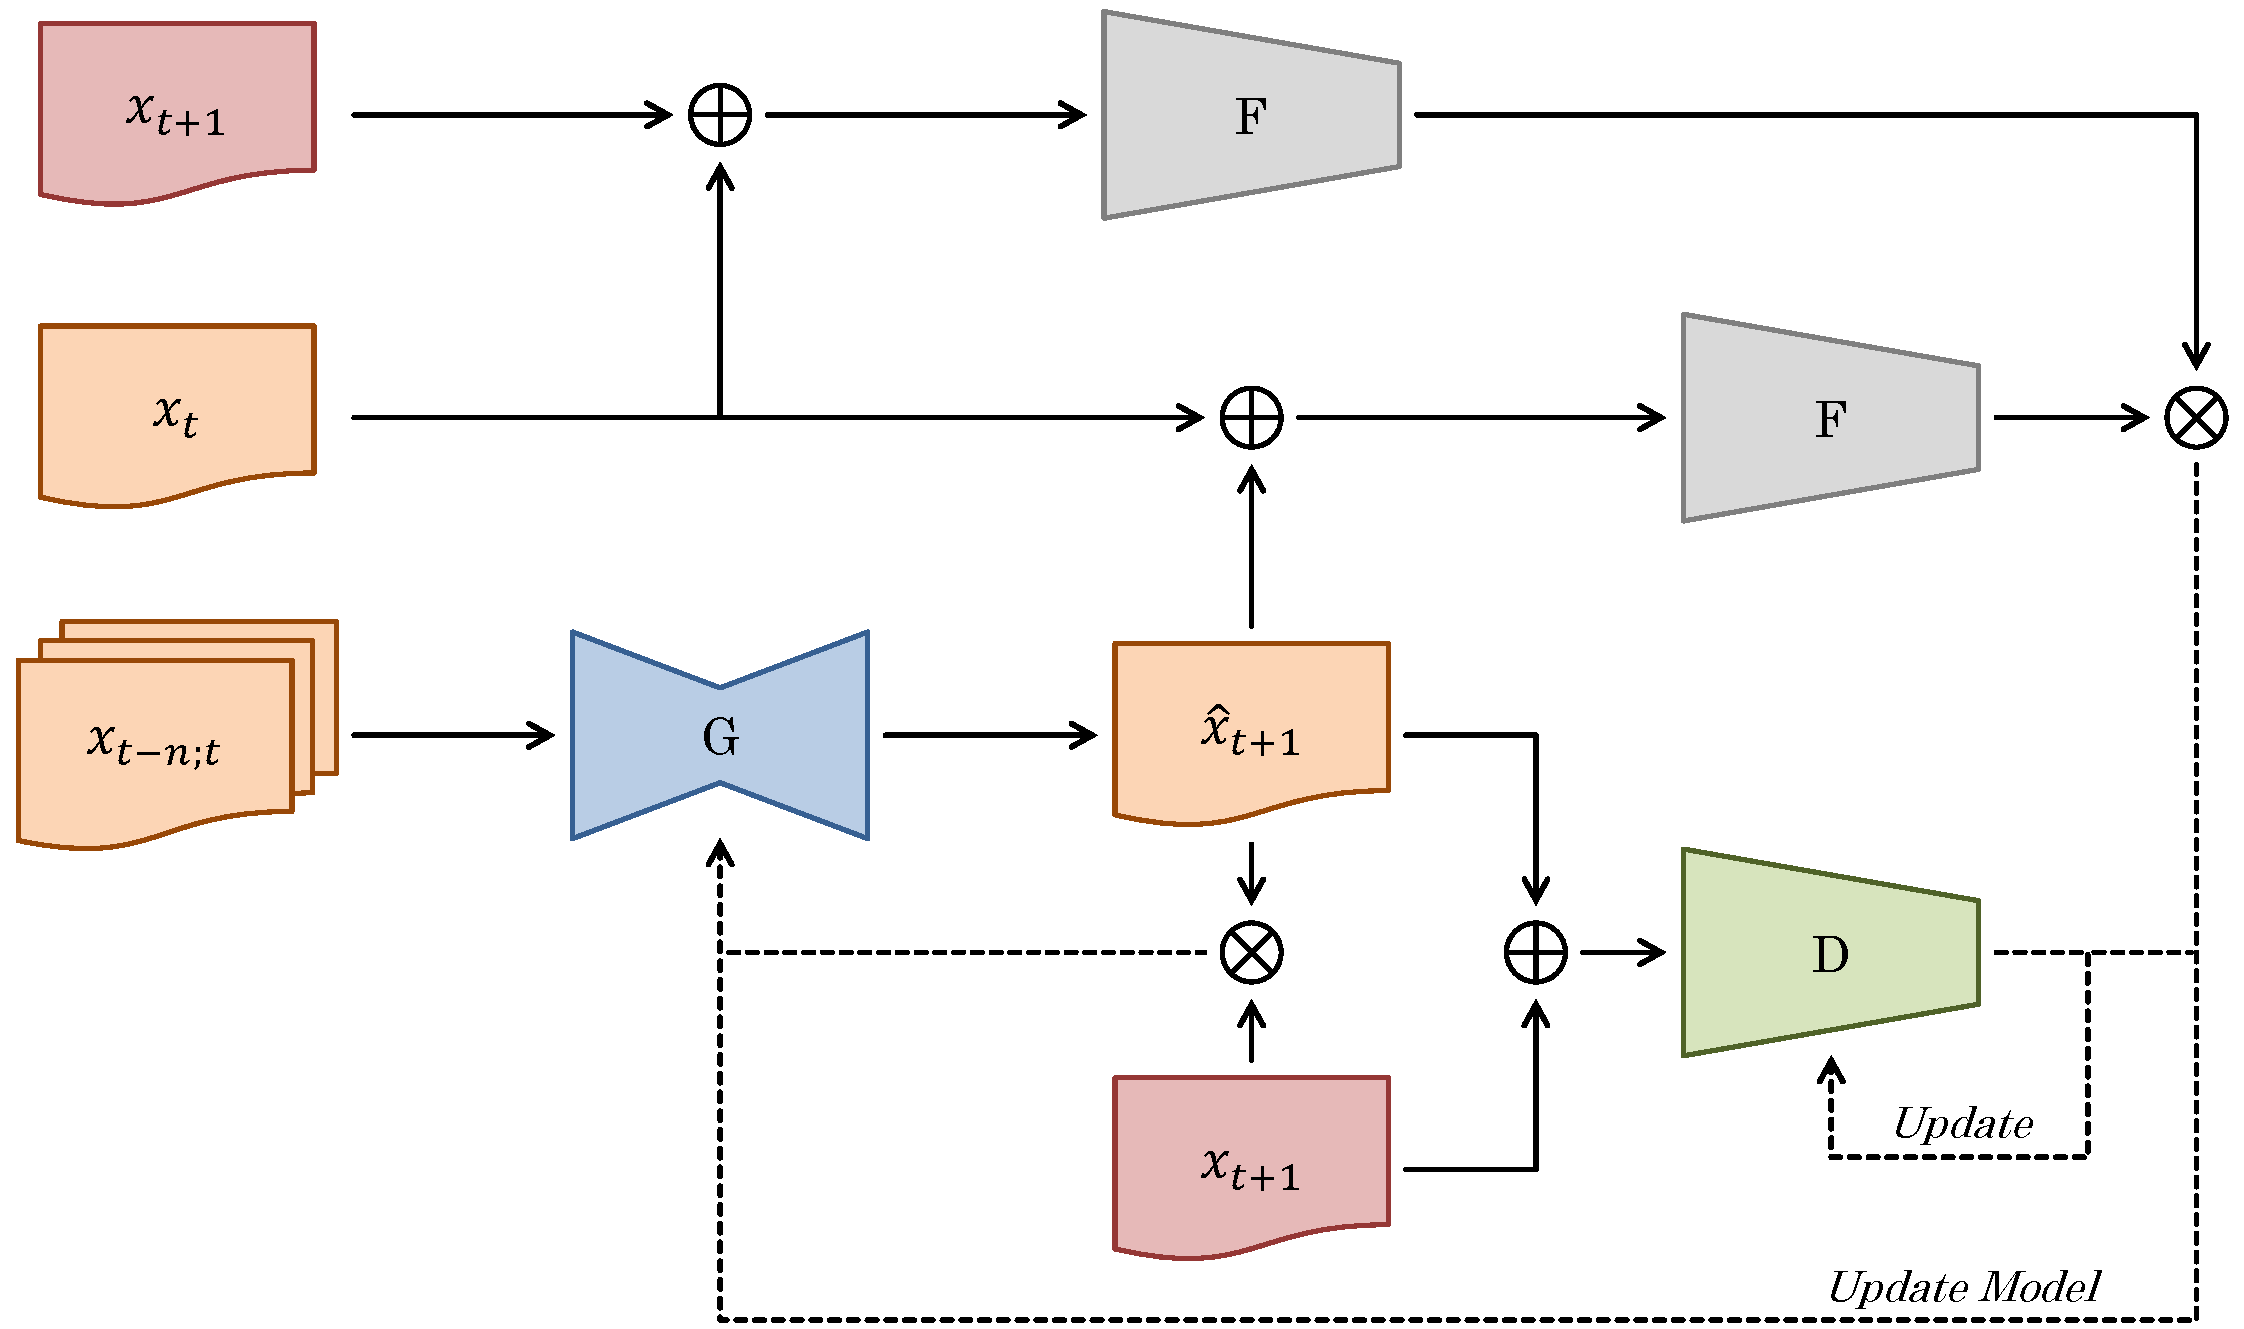
\includegraphics[width=1\textwidth]{graphics/gan/unet/unet.pdf}
  \caption[U-Net-based generative future frame prediction architecture.]{U-Net-based generative future frame prediction architecture \cite{liu2018future}. Training the generator ($G$) is done both adversarially with a spatial CNN as discriminator ($D$), and directly; overall appearance and motion of a predicted frame are enforced through separate loss terms ($\bigotimes$) and an auxiliary optical flow network ($F$).}
  \label{fig:u_net}
\end{figure}

Recently, different kinds of solutions for anomaly detection for video have been presented, using generative future frame prediction models as we do. Like our approach, these models are trained in unsupervised manner on mostly normal data under the assumption, that they will only be able to make correct predictions on normal videos, while not being able to find accurate representations for anomalous video frames. Therefore leveraging the computable difference between a predicted future frame and the actual one to detect an anomalous event. However unlike the IFTM framework that we adapted and utilized (see Section \ref{sec:vad}), they lack an adaptive threshold model (TM). On the other hand, some of their modified GAN architectures feature additional components and loss terms, to increase the prediction quality; similar to the architectures presented in the previous two sections of this chapter.

% liu2018future uses mahadevan2010anomaly GAN
Liu et al. propose a next-frame video prediction architecture, shown in Figure \ref{fig:u_net}, that they use for anomaly detection \cite{liu2018future}. Like other video generation and prediction approaches mentioned earlier, they utilize the U-Net architecture for the generator, which is an one-stream 3D CNN encoder-decoder, featuring skip connections between intermediate encoding and decoding layers \cite{ronneberger2015u}. In addition, they also untangle motion and appearance, though this is not accomplished by explicitly modeling the generator network that way. Instead loss terms were added for optical flow, intensity, and gradient loss. The former enforces realistic motion. This is achieved, not using the discriminator like in VOS-GAN or FTGAN (see Section \ref{sec:rel_vgan}), but through a separate pretrained version of Flownet \cite{dosovitskiy2015flownet}. The network is used to calculate the optical flow of a frame pair consisting of the current frame and either the actual next frame or the predicted one, with the loss being the L1 distance between the two flows. Intensity and gradient generator loss, enforcing appearance quality, are also computed by comparing the predicted frame to the ground truth. This makes the discriminator somewhat redundant and reduces the generator's generalization capabilities --- same was the case for MCnet, since it is no longer indirectly trained in its task; this goes against one of the reasons why GANs are used in the first place as explained in Section \ref{sec:gans}. The discriminator only serves to improve the general realness of the predicted next frames and does not enforce temporal consistency. After training has been completed, predicted test frames are compared to their ground truth counterparts using the peak signal to noise ratio (PSNR)\nomenclature{PSNR}{Peak signal to noise ratio} to perform anomaly detection. However Liu et al. do the detection phase offline, since the PSNR values of all frames in the test set are normalized, before they manually set the threshold to distinguish normal and anomalous frames.

% jamadandi2018predgan uses mahadevan2010anomaly GAN
Detecting anomalies using a threshold and the PSNR values is done under the assumption, that when a prediction network encounters anomalous frames, the generated frames consist of fuzzy regions in which the anomalous object patterns are taking place. These fuzzy frames have lower PSNR values than their ground truth counterparts. Jamadandi et al. build on that premise and develop it further using their video prediction framework called PredGAN \cite{jamadandi2018predgan}. Their GAN architecture however makes predictions for a number of future frames equal to the number of input frames at each step. And unlike in the previous architecture, the discriminator --- a 3D CNN, rates the realness of both appearance and motion in the video, like in our modified version of C-VGAN (see Section \ref{subsec:vgan_mod_2}). For the generator, Jamadandi et al. employ a multiscale network to prevent loss of resolution and long-range dependencies. Such a CNN accepts the input video frames at differently scaled versions, later combining them linearly \cite{mathieu2015deep}. To train such a model for prediction, besides adapted GAN loss terms for generator and discriminator to account for the multi-scale generator architecture, both the L1 and L2 distance between actual and predicted frames of the generator are directly minimized. Again, the discriminator is reduced to an auxiliary component, not indirectly training the generator for prediction anymore. After the offline training phase has been completed, to use the future frame prediction generator model for anomaly detection, Jamadandi et al. propose to use the Earth Mover's Distance (EMD)\nomenclature{EMD}{Earth mover's distance} --- also known as the Wasserstein metric, instead of PSNR. EMD is a metric to evaluate the dissimilarity between the actual and predicted video frames. They reason, that EMD captures the perceptual similarity better, being closer to the human vision system. However, while achieving similar evaluation results to Liu et al. \cite{liu2018future}, they still offer no way of automatically setting the threshold to determine whether a frame is anomalous or normal. Again it needs to be set by an expert after obtaining all normalized EMD scores for the test set.

% dong2020dual uses mahadevan2010anomaly GAN
Forcing the generator to make a next-frame prediction exactly to the ground truth through the explicit definition of the prediction loss, comes at the already mentioned cost of generalization capabilities. Dong et al. face this issue as well and they try to remediate it via a dual discriminator GAN architecture \cite{dong2020dual}: Similar to MoCoGAN and AMC-GAN from the previous sections, one spatial CNN rates the realness of a given predicted frame, while the motion discriminator distinguishes real and synthetic videos. To avoid the motion discriminator defaulting to discriminate the videos based on appearance patterns, it only gets the optical flows of both real and fake videos. As in Liu et al. \cite{liu2018future}, they estimate the flow using a pre-trained version of FlowNet, passing it to the motion discriminator. But their architecture mirrors the one by Liu et al. further, also directly defining flow, intensity, and gradient loss. How Dong et al. set the loss term weights during training is not mentioned. Thus it is unclear, how much of an influence the adversarial training and the two discriminators actually have on the generator model. The generator is once more a one-stream U-Net encoder-decoder, with the attached disadvantages of not untangling motion and content of a video. For anomaly detection PSNR is utilized again, with no mention on how to set the threshold.

% nguyen2020anomaly uses ai2029dataset GAN
Nguyen et al., same as the previous approach, do not propose a novel method, but utilize the framework of Liu et al. \cite{liu2018future}, but they replace the input video for the generator with a motion encoded image \cite{nguyen2020anomaly}:  This is done by averaging the input frames' pixel values using an exponential moving average, emphasizing the more recent past more in a given video. Further, the generator, which still is a U-Net-based encoder-decoder, gets the motion encoded image and the frame of the current time step, to extrapolate the next frame. This is similar to the generator of AMC-GAN from the previous section, allowing the generator to more focus on making the prediction and not wasting its capacity on the encoding of trajectory information like in other approaches. In addition, Nguyen et al., replace the intensity loss function with a scaled one, since their use case is CCTV traffic footage, with lots of fast-moving object patterns. Training of the model is again done offline, before anomaly detection is done using PSNR and a custom threshold to distinguish between normal and anomalous frames.

For evaluation, the first three proposed approaches computed the receiver operation characteristic (ROC)\nomenclature{ROC}{Receiver operation characteristic} curve, by gradually changing the threshold for the computed PSNR or EMD scores on the test set, and measuring the resulting true and false positive rates \cite{liu2018future, jamadandi2018predgan, dong2020dual}. They then leveraged the resulting area under the ROC curve (AUC)\nomenclature{AUC}{Area under the curve}, cumulating it into a scalar, for anomaly detection evaluation. All of them performed such an evaluation mainly on the UCSD anomaly detection pedestrian dataset \cite{mahadevan2010anomaly}. The data set was acquired using a stationary camera, overlooking pedestrian walkways, with anomalies being naturally occurring events, such as small cars driving on the walkway. On the other hand, Nguyen et al. did not use ROC and AUC, but a custom evaluation metric, that consisted of an aggregration of the F-Measure and a detection time error \cite{nguyen2020anomaly}. Their evaluation was done using the anomaly detection data set from the AI City challenge 2019, featuring 100 videos of traffic for training and testing each, with a total of 50 hours of material \cite{ai2029dataset}.

The overarching issue of these four approaches is --- no matter their underlying prediction model and their performance, that none of them mentions how to set the threshold. It is often an afterthought. And, while ROC and AUC are legitimate metrics to evaluate a model's performance \cite{bradley1997use}, it is not a sufficient indicator on how the detection model would perform on a continuous video frame stream. As explained in the presentation of our use case in Section \ref{sec:use_case}, the detection phase only allows the processing of each frame exactly once. Meaning, a threshold can not be set after the anomaly scores of the entire test set have been computed and normalized. It either has to be set in advance or be continuously adapted over time. For the evaluation of the approach by Nguyen et al. \cite{nguyen2020anomaly}, there is an even greater issue, since their utilized metric is based on the results of a single configuration's confusion matrix like ours (see Section \ref{subsec:vad_eval_method}), using a unmentioned threshold. It is even brought up by them, that only the PSNR scores from a single video determine the threshold that is applied to the scores of that video. Meaning, that the threshold maximizes their selected evaluation score, since the true labels are already known. No validation in any form is performed. In addition in the real world, these large amounts of data are usually not labeled and it would require domain expertise to set a threshold that way. Even then, the threshold can only be set offline based on the available training data and not on the unknown evaluation data set. Like our ADS for video using IFTM, which is able to operate on a continuous video stream in real-time during the detection phase, after it has approximated the threshold in offline manner using the training data set.

\paragraph{Reconstruction-Based}

\begin{figure}
	\centering
	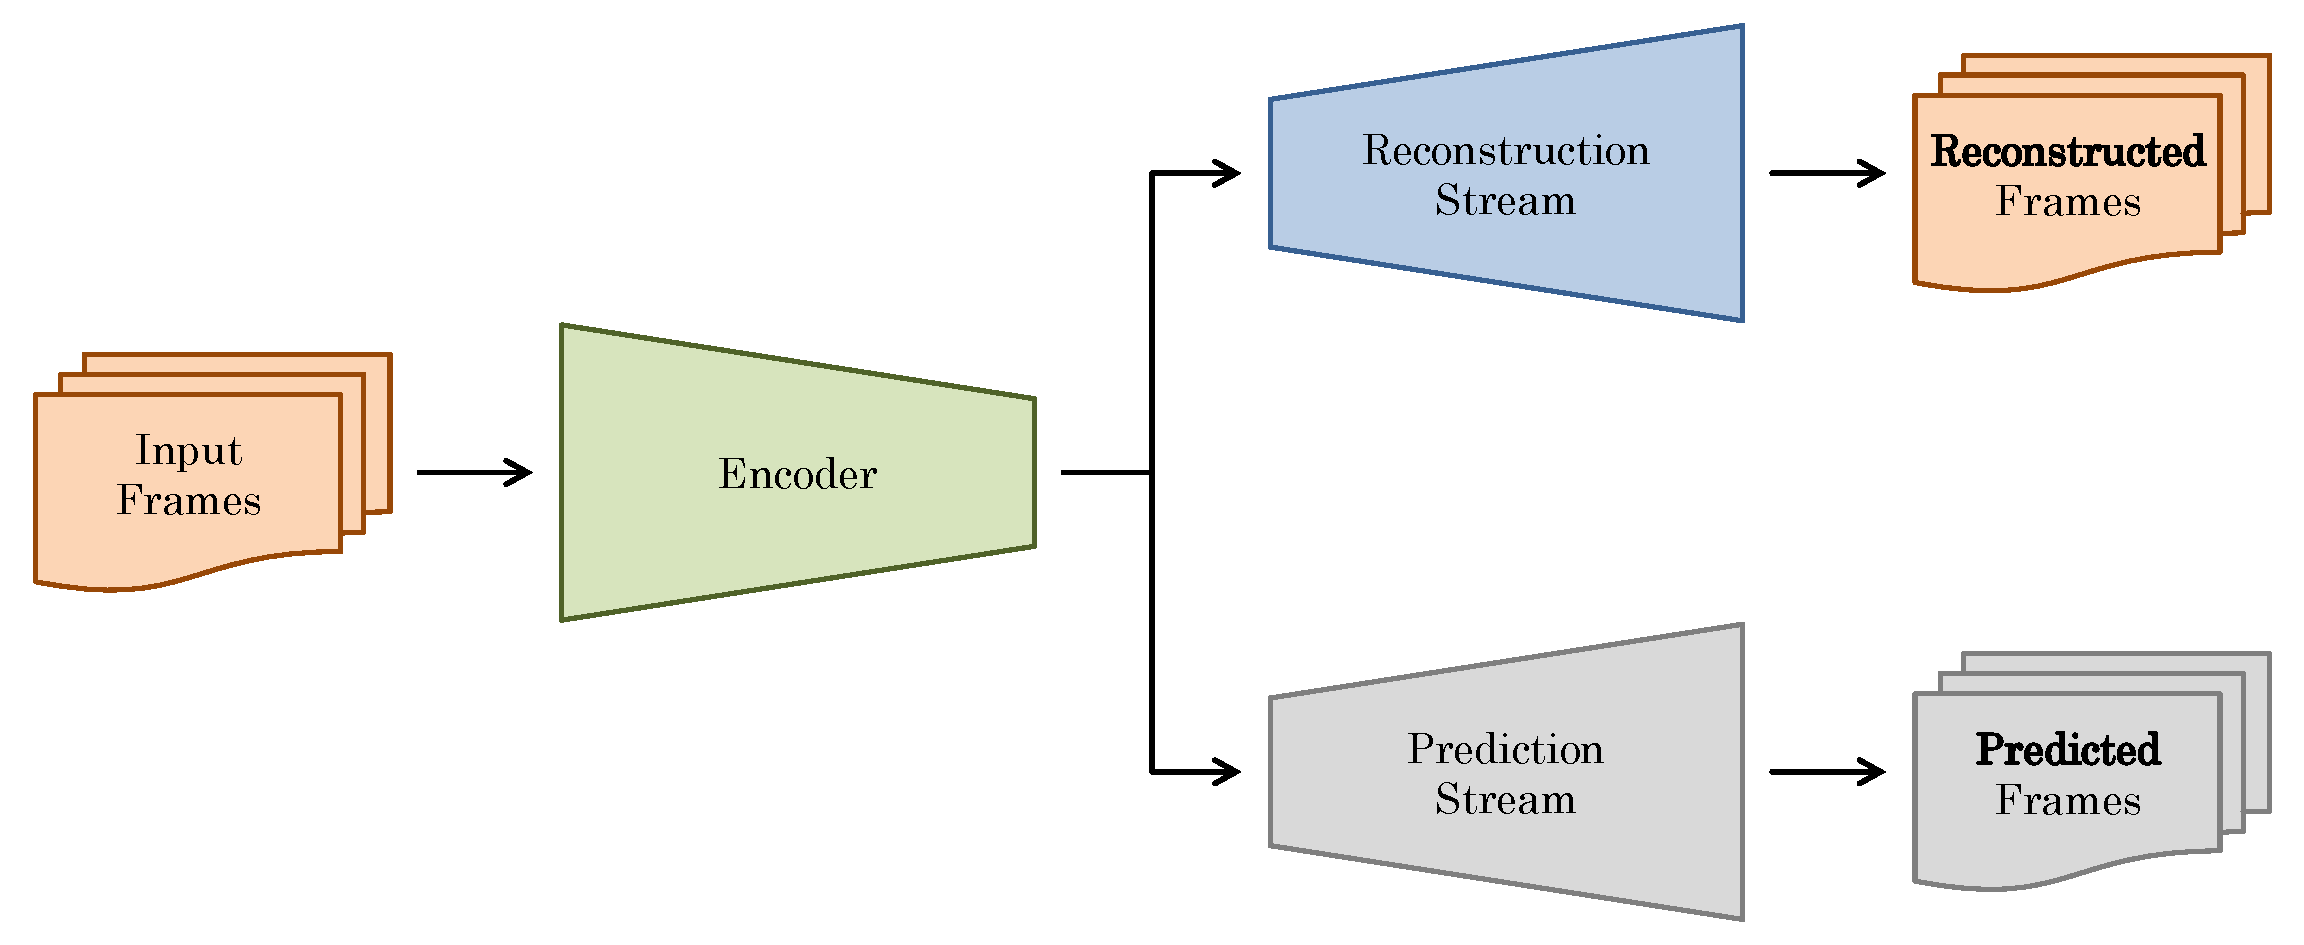
\includegraphics[width=1\textwidth]{graphics/gan/convAE/convAE.pdf}
  \caption[Spatio-temporal convolutional autoencoder using two decoder pathways.]{Spatio-temporal convolutional autoencoder using two decoder pathways \cite{zhao2017spatio}. Because both share the same encoder, the auxiliary pathway for future frame prediction guides the model to extract temporal features.}
  \label{fig:auto_enc}
\end{figure}

% uses mahadevan2010anomaly autoencoder with reconstructions + prediction? 
For many of the mentioned GANs in this section, the discriminator often is only an auxiliary component, with the task of the generator being optimized directly using appearance and motion losses. Zhao et al. go one step further, abandoning the adversarial concept but extending the model in a different way \cite{zhao2017spatio}: First, their goal is not to detect anomalies by comparing a predicted future to the actual one, but to reconstruct given input frames like an identity function. Consequently, frames are classified based on their reconstruction error; this is again under the assumption, that a model trained using mostly normal data, will be able to find a representation for normal data but not for anomalous one. Thus a spatio-temporal autoencoder is utilized, as depicted in Figure \ref{fig:auto_enc}. It first encodes a given video into its latent representation using a one-stream 3D CNN. Afterwards however, two separate pathways decode the latent information for either reconstruction or future frame prediction. While irrelevant for the detection phase, Zhao et al. argue, that a normal autoencoder would not be able to learn to encode the trajectory information of object patterns. Extending the model's task to future frame prediction, forces the one-stream encoder to focus on temporal features, which is necessary when one wants to detect anomalous motion patterns; see Section \ref{subsec:anomaly_types} for the types of anomalies found in video. For training the model, reconstruction and prediction loss are minimized. The former is expressed using the mean square error over all the given frames, while the latter is a adjusted weight-decreasing prediction loss. They argue, the more steps one takes into a predicted plausible future, the more it potentially deviates from the actual one. For example, new object patterns can appear, while old ones might leave a scene. Thus the prediction loss function weights the first frame of a predicted series more, linearly decreasing the weights of successive frames.

For anomaly detection, after the model has been trained, the reconstruction error of a sequence of frames is defined using the reconstruction loss from training. The resulting score is then normalized for the entire test video, as it was done for the prediction-based approaches presented before in this section. However Zhao et al. unlike others note that such a detection method is impractical for the real world and advise to calculate the minimum and maximum reconstruction error experimentally on historical data, so one can compute the errors and normalize them for new videos in real-time. For anomaly detection evaluation, the UCSD anomaly detection pedestrian dataset \cite{mahadevan2010anomaly} was used again. However, evaluating their proposed system using AUC and the equal error rate (EER)\nomenclature{EER}{Equal error rate}, Zhao et al. offer no insight on how to set the threshold, that maps the reconstruction error scores to the binary classes. The system would still require a human expert to define a domain specific threshold, or one would need to use a separate threshold model to fulfill the detection task.

\paragraph{Adversarial Transfer Learning}

% uses mahadevan2010anomaly GAN
Finally, not every ADS for video is trained in unsupervised mode. There are others that get access to the true labels directly, to either fully train or refine their model at a later stage of the training procedure. Shin et al. \cite{shin20203d} propose a multi-step training process: In the first step, a GAN featuring a U-Net-based autoencoder as generator creates synthetic reconstructions of given input frames, with the discriminator, a 3D CNN encoder with LSTM components, rates them as either real or fake. The value function optimized during adversarial training is not modified. Thus that training training is unsupervised as usual. Then in the second training phase, the first half of the autoencoder, computing the latent representation of a video, is transferred to a VAD classifier. It is disconnected from the model and then refined for VAD using a small but labeled data set. They argue, that for the initial training of the classifier, there is not enough labeled training data available. But, under the assumption, that during the first phase, the model learned to represent only normal data since it was mostly trained on that class, the tasks of generation and classification overlap. In addition, a fully connected neuron is attached to the end of the classifier, so there is only one output value, ranging from $0$ to $1$. This corresponds to the anomaly score of an input video and no reconstruction or prediction error function need to be used. Further, Shin et al. set the threshold to map the score to binary labels using the EER, where the false positive and false negative rate are equal for the available labeled training data set.

Evaluation was done using the UCSD pedestrian datasets \cite{mahadevan2010anomaly}. They evaluated their model's generalization capabilities using 10-fold cross validation and they compared it to earlier work of supervised VAD models. Their model showed the highest accuracy across validation folds, but having a slightly lower EER and AUC score. During the analysis of the misclassified video samples, they note that the model struggles especially with anomalies not encountered during training. It is a common problem across application domains, when one has a labeled but limited training data available that is not fully representative of the test set but one has to learn all existing classes; see Section \ref{subsec:detection_techniques} for the different types of anomaly detection techniques. Note that this can also happen when training in unsupervised manner, if there are unknown normal states, which will look like anomalies to the ADS. Though diverse mostly normal data is often more readily available than labeled data containing both classes. Lastly --- this includes other presented models in this section that were utilized for VAD as well, for the purpose of video generation and prediction, a one-stream generator is often considered to be suboptimal. Approaches that explicitly untangle motion and content through their network architecture, such as presented in Section \ref{sec:rel_vgan} and \ref{sec:rel_frame_prediction} but also VGAN, were often compared to one-stream baselines in their evaluation, outperforming all of them by wide margins. Because when encoding for example an unknown motion in a known scene, a one-stream generator might find no suitable latent representation for it. Meanwhile in a two-stream approach, the motion might be known in another context, which would allow the model to generalize from that scene to the given one. Such an architecture, when applied for adversarial transfer learning to VAD, would also help with the generalization and classification problem of unencountered data during training.